\chapter{How I Turned \$1,000 Into \$1 Billion}

This chapter follows Glen Boyd's School of Hard Knocks interview, curated by LazyingArt LLC, as a source of business mechanics rather than as a recipe. The interview begins with the result and then works backward: a small security-software company, a sudden internet pivot, rapid customer proof, difficult financing choices, and the operating discipline needed to survive scale. The mathematics here is not formal physics. It is the arithmetic of validation, runway, ownership, and capacity.

\section{The Result Before The Mechanism}

Boyd opens with the proof-point before the origin story. The new product did \(\$50{,}000\) in business in the first month without advertising, nearly caught the old security business within eleven months, and reached \(\$120{,}000{,}000\) in sales within four years. Written as a growth trace, the claim is:

\begin{equation}
\$50{,}000\ \text{in month 1}
\;\longrightarrow\;
\text{near the old security business by month 11}
\;\longrightarrow\;
\$120{,}000{,}000\ \text{in sales by year 4}.
\end{equation}

That equation is not an explanation. It is the thing to be explained. The interview then backs up to the starting conditions: Boyd taught himself programming, started young, built EG Software, took the company public in 1999, and later sold it in a merger. The larger point is already visible. The billion-dollar outcome did not begin as a billion-dollar idea. It began as a useful technical capability in a narrow institutional market.

\section{From Security Logs To Marketing Signals}

The original product was a security product for local-area networks. Boyd describes it as a kind of surveillance and audit-control system for internal networks at a time when the internet was not yet widely used. Banks and financial institutions needed to know what was happening inside their computerized systems. The product logged and analyzed traffic and access on those networks.

The first mechanism was:

\begin{equation}
\text{local-area-network traffic}
\;\longrightarrow\;
\text{logging and analysis}
\;\longrightarrow\;
\text{security or audit report}.
\end{equation}

This was not merely an idea. Boyd says the company had the Federal Reserve, almost every major bank in the United States, and a four-person team doing roughly \(\$1{,}000{,}000\) per year from a small office. The owned asset was the analysis engine: software that could process large amounts of traffic quickly.

Then the field changed. Yahoo and Netscape appeared. The whole world was becoming networked. Boyd's question became the natural one:

\begin{equation}
\text{existing analysis engine}
+
\text{new internet traffic}
\;\Longrightarrow\;
\text{new commercial use?}
\end{equation}

\begin{figure}
\centering
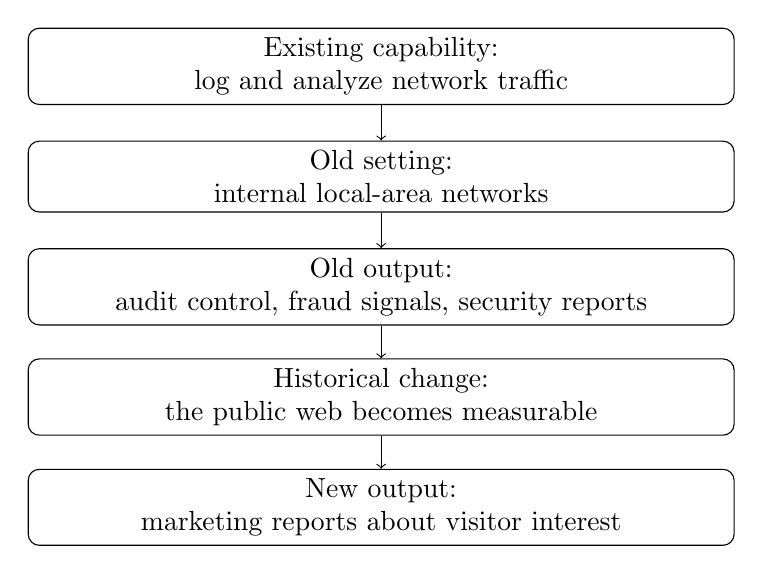
\begin{tikzpicture}[x=1cm,y=1cm]
\node[draw, rounded corners, align=center, text width=.72\linewidth] (a) at (0,0) {Existing capability:\\log and analyze network traffic};
\node[draw, rounded corners, align=center, text width=.72\linewidth] (b) at (0,-1.40) {Old setting:\\internal local-area networks};
\node[draw, rounded corners, align=center, text width=.72\linewidth] (c) at (0,-2.80) {Old output:\\audit control, fraud signals, security reports};
\node[draw, rounded corners, align=center, text width=.72\linewidth] (d) at (0,-4.20) {Historical change:\\the public web becomes measurable};
\node[draw, rounded corners, align=center, text width=.72\linewidth] (e) at (0,-5.60) {New output:\\marketing reports about visitor interest};
\draw[->] (a) -- (b);
\draw[->] (b) -- (c);
\draw[->] (c) -- (d);
\draw[->] (d) -- (e);
\end{tikzpicture}
\caption{The pivot reused the same analytic capability in a different market.}
\end{figure}

Boyd's key transformation can be stated as a before-and-after:

\begin{align}
\text{security product}
&:\quad
\text{local traffic} \longrightarrow \text{security report},\\
\text{web analytics product}
&:\quad
\text{anonymous web traffic} \longrightarrow \text{marketing report}.
\end{align}

The example from the interview is Sports Illustrated. A website owner did not merely need a hit count. They needed to know whether \(100{,}000\) people were visiting once or \(10{,}000\) people were returning ten times. The customer problem was measurement, and Boyd already had a machine built for measurement.

\subsection{Question \& Answer}

\paragraph{Question.}
How did Boyd know this was the thing to go all in on?

\paragraph{Answer.}
He did not know as a proof. He saw a discontinuity. The internet was the train going by, and the practical judgment was that they might catch the last car if they ran immediately. The risk was that they would redirect a successful small business. The payoff was that their existing technology could answer a new and urgent question.

The market supplied the resolution:

\begin{equation}
\text{uncertain pivot}
\;\longrightarrow\;
\$50{,}000\ \text{without advertising in month 1}
\;\longrightarrow\;
\text{validated demand}.
\end{equation}

That is the rhythm of the first part of the interview: not certainty, then action, then success; rather, useful capability, historical change, risky pivot, and customer proof.

\section{The Adoption Test}

When the interviewer turns to funding, Boyd does not begin with valuation or pitch language. He begins with demonstration. Ideas are hard to fund. A sample or partial product goes further. A product that people are already using goes further still.

He calls this the dog-food test: will people actually use the product? In compact form:

\begin{equation}
\text{idea}
\;<\;
\text{demonstrable product}
\;<\;
\text{product with early adoption}.
\end{equation}

Or, as an operating rule reconstructed from his answer:

\begin{equation}
\text{idea}
+
\text{demonstrable product}
+
\text{early adoption}
\;\Longrightarrow\;
\text{credible funding path}.
\end{equation}

\paragraph{Worked example.}
Suppose three founders approach an investor.

\begin{enumerate}
\item Founder A has only the claim that people will want the product.
\item Founder B has a working sample.
\item Founder C has a working sample and repeated early usage.
\end{enumerate}

Let \(U\) denote investor uncertainty about demand. Boyd's rule says the uncertainty decreases in this order:

\begin{equation}
U_A > U_B > U_C.
\end{equation}

This is why the early revenue in Boyd's story matters. It is not decorative. It answers the first financing question: whether the market is pulling on the product.

\section{Risk, Health, And The Partner Constraint}

The interview then widens from product proof to personal survivability. Boyd says entrepreneurship made work-life balance difficult, and later, as he got older, the problem became life-health-work balance. He had children young, built a high-growth company young, went through divorce, and later had a heart attack and triple bypass surgery. The chapter should not turn this into generic wellness advice. In Boyd's account, health and relationships are operating constraints.

That is where the partner enters the mechanism. A strong co-partner was not only emotional support. It was a way to divide work, cover emergencies, and bring skills that one founder did not have. Boyd also emphasizes trust under conflict: honest people, intelligent people, and people who can take constructive feedback, including oneself.

The concrete risk story is stark. He had a newborn on the way, quit his job, wrote the first product, and got down to about \(\$1{,}000\) in the bank. He sold his motorcycle, which bought another month or two. Then his partner put in personal money.

\begin{equation}
\$1{,}000\ \text{left}
+
\text{motorcycle sale}
+
\text{partner cash}
\;\longrightarrow\;
\text{survival runway}.
\end{equation}

The risk model was not that failure was impossible. It was that failure had a floor:

\begin{equation}
\text{business failure}
\;\longrightarrow\;
\text{go get a job}.
\end{equation}

The regret model pointed the other way:

\begin{equation}
\text{do not try}
\;\longrightarrow\;
\text{years of wondering why not}.
\end{equation}

That pair of equations is the practical psychology of the risk. One side bounded the downside; the other made inaction costly.

\section{Bad Fit, Venture Capital, And Ownership}

Boyd's worst financial decision was entering a business he did not want to be in. He describes a construction loan, collateral, failing management, several years spent turning the situation around, a tragic accident, and a loss close to \(\$3{,}000{,}000\). The lesson is deliberately plain: do not get involved in something you do not want to be involved in, especially when your instinct says no.

The interview then flips to his best financial decision. The company was profitable and growing quickly. Boyd and his partner wanted capital to expand faster, so they courted a venture-capital firm. The process took energy and attention. The firm eventually passed.

\begin{figure}
\centering

\includegraphics[width=\linewidth]{lecture_16_figure_05.png}
\caption{Startup-pitch imagery beside Boyd's discussion of courting venture capital. The visible board text reads ``START UP,'' but the ownership claim comes from the spoken interview, not from the small unreadable charts in the frame.}
\end{figure}

\subsection{Question \& Answer}

\paragraph{Question.}
Why would a failed financing process become the best financial decision?

\paragraph{Answer.}
Because the failure changed the ownership equation. No venture capital meant no financial cushion. It also meant more frugal decisions and less dilution. Boyd says that when the company went public, he and his partner owned \(95\%\) of it.

\begin{figure}
\centering
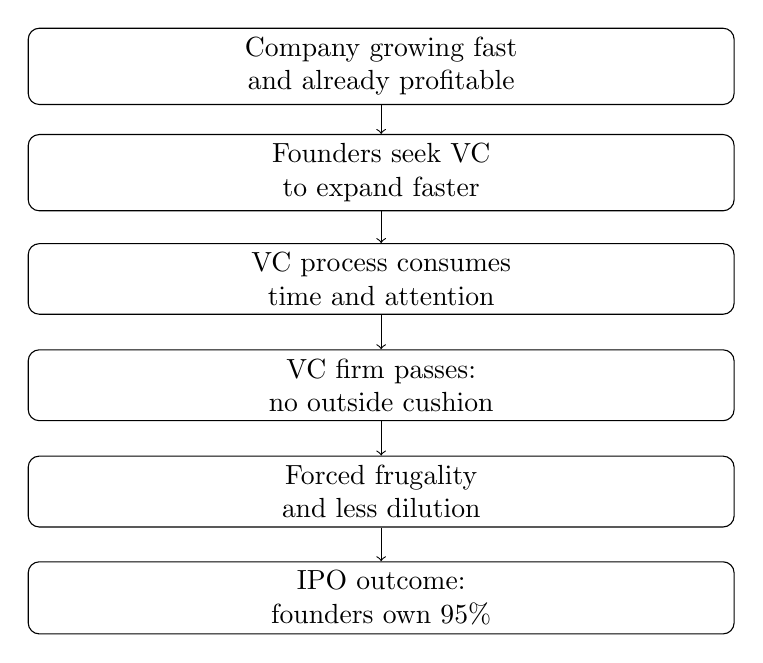
\begin{tikzpicture}[x=1cm,y=1cm]
\node[draw, rounded corners, align=center, text width=.72\linewidth] (a) at (0,0) {Company growing fast\\and already profitable};
\node[draw, rounded corners, align=center, text width=.72\linewidth] (b) at (0,-1.35) {Founders seek VC\\to expand faster};
\node[draw, rounded corners, align=center, text width=.72\linewidth] (c) at (0,-2.70) {VC process consumes\\time and attention};
\node[draw, rounded corners, align=center, text width=.72\linewidth] (d) at (0,-4.05) {VC firm passes:\\no outside cushion};
\node[draw, rounded corners, align=center, text width=.72\linewidth] (e) at (0,-5.40) {Forced frugality\\and less dilution};
\node[draw, rounded corners, align=center, text width=.72\linewidth] (f) at (0,-6.75) {IPO outcome:\\founders own \(95\%\)};
\draw[->] (a) -- (b);
\draw[->] (b) -- (c);
\draw[->] (c) -- (d);
\draw[->] (d) -- (e);
\draw[->] (e) -- (f);
\end{tikzpicture}
\caption{The rejected financing round becomes valuable because it preserves ownership and imposes discipline.}
\end{figure}

The compact ownership mechanism is:

\begin{equation}
\text{sought VC}
\;\longrightarrow\;
\text{VC passed}
\;\longrightarrow\;
\text{frugality}
\;\longrightarrow\;
95\%\ \text{founder ownership at IPO}.
\end{equation}

The point is not that venture capital is bad. The point is that financing changes the shape of the cap table and the behavior of the company. In Boyd's case, the absence of outside capital forced discipline and preserved the claim on the upside.

\section{Scaling Until People Run Out Of Oxygen}

Boyd's first scaling rule is expense control. As a business grows, expenses also grow; the numbers become multiples. A single bad dip can wipe out a company whose cost structure has outrun its resilience.

Then he gives the more memorable scaling model from \emph{Into Thin Air}. At altitude, even tying one's shoes can become difficult. Different people have different limits. Some can climb higher; some need support; some must come down the mountain. Boyd maps this directly onto management capacity in a fast-growing company.

An employee may be excellent at one altitude:

\begin{equation}
4\text{--}10\ \text{direct reports}.
\end{equation}

Six months or a year later, the same person may be at a new altitude:

\begin{equation}
20\text{--}30\ \text{direct reports}
\;\longrightarrow\;
\text{capacity failure risk}.
\end{equation}

This gives an explicit hiring rule. If \(R\) is the current role and \(\Delta R\) is the predictable increase in responsibility, then hiring only for \(R\) is not enough:

\begin{align}
\text{current role} &= R,\\
\text{near-future role} &= R+\Delta R,\\
\text{required capacity} &\geq R+\Delta R.
\end{align}

In Boyd's language, hire someone who has already been up the mountain. If the role is \(20\) people today but will be \(50\) people within a year, the candidate should already have operated at that level.

\begin{table}
\centering
\small
\begin{tabular}{|p{.22\linewidth}|p{.28\linewidth}|p{.34\linewidth}|}
\hline
\textbf{Growth state} & \textbf{Failure signal} & \textbf{Management response} \\
\hline
Employee succeeds at present scale & Work fits current capacity & Keep responsibility matched to role \\
\hline
Company grows quickly & Same person now carries a larger span & Stop adding balls; reduce or divide responsibility \\
\hline
Future role is predictable & Candidate has not operated at that altitude & Hire above the current level \\
\hline
\end{tabular}
\caption{Boyd's altitude metaphor converted into an operating table for scaling responsibility.}
\end{table}

Boyd also mentions \emph{Crossing the Chasm} as a useful marketing frame for launching new products into new markets. In the order of the interview, that book appears after the altitude lesson, and it returns us to the earlier adoption problem: a product must cross from early interest into broader market acceptance.

\section{Money, Advice, And The Last Constraint}

After the sale, the interviewer asks whether money buys happiness. Boyd's answer is bounded. Money helps when it moves someone from poverty toward security: paying bills, sending children to college, and having freedom to try new things. Past a certain level, more money does not keep buying more happiness.

As a curve, the claim is not linear:

\begin{equation}
\text{value of additional money}
\;\text{rises sharply near insecurity and flattens after basic freedom}.
\end{equation}

His younger-self advice follows from that shape. Enjoy life more. Maybe finish college. Build deeper relationships. Take care of health before it becomes the easiest thing to neglect. Do not spend too much once money arrives. Get serious financial advice.

The final rule is about time. Boyd calls procrastination the enemy because time is not renewable. If failure is likely somewhere in an entrepreneurial life, the better strategy is to fail fast, learn, and move.

\begin{equation}
\text{delay}
\;\longrightarrow\;
\text{later learning}
\;\longrightarrow\;
\text{greater distance from success}.
\end{equation}

And the positive version is:

\begin{equation}
\text{start}
\;\longrightarrow\;
\text{test}
\;\longrightarrow\;
\text{fail or validate}
\;\longrightarrow\;
\text{adjust faster}.
\end{equation}

\section{Summary}

The interview's spine is a chain of mechanisms. Boyd begins with a narrow but real security product. The internet changes the field. The company reuses its traffic-analysis engine, turning security reports into marketing reports. Early customers validate the pivot. Funding becomes a question of demonstration and adoption. Risk becomes survivable through runway, a fallback, and a partner. A failed venture-capital courtship preserves ownership and enforces frugality. Scale then creates a new bottleneck: people and expenses can exceed their operating altitude.

The durable mechanism is:

\begin{equation}
\text{technical capability}
\;\longrightarrow\;
\text{market pivot}
\;\longrightarrow\;
\text{customer validation}
\;\longrightarrow\;
\text{disciplined financing}
\;\longrightarrow\;
\text{retained ownership}
\;\longrightarrow\;
\text{durable wealth}.
\end{equation}

That is the chapter's main claim. The money came after a sequence of judgments: what to reuse, when to pivot, how to prove demand, what risk to bear, what capital not to take, and how to keep the company from breaking as it climbed.